\setchapterimage[6.5cm]{Grid_FullView_Logo}
\setchapterpreamble[u]{\margintoc}
\chapter{IceCube Realtime Alerts}
\labch{realtime}
\begin{fquote}[Alan Turing][Computing Machinery and Intelligence][1950]A very large part of space-time must be investigated, if reliable results are to be obtained. Otherwise we may (as most English children do) decide that everybody speaks English, and that it is silly to learn French.
\end{fquote}

As a complement to the Likelihood analysis methods introduced in Chapter \ref{ch:llh}, neutrino astronomy can also be conducted through \emph{realtime} analysis in which automated neutrino alerts are published with low latency. These public neutrino alerts can then be \emph{followed-up} by external observatories, in order to search for possible photon counterparts. This latter aspect is explained in more detail in Chapter \ref{ch:ztf_too}, where one such follow-up program with the Zwicky Transient Facility (ZTF) is outlined.

In this chapter, the IceCube Realtime Program is introduced. As part of this thesis, the author maintained and further developed the IceCube Realtime System from October 2018 to mid 2020, acting as first responder to the vast majority of neutrino alerts in that period.

\section{Realtime Multi-Messenger Astronomy}

In recent years, there has been a significant interest in the study of transient and variable objects in astronomy (see also Chapter \ref{ch:sources}). Driven primarily by the speed at which objects can evolve and disappear, particularly GRBs and latterly Kilonovae, it is often essential that astronomy can be done with minimal latency. In this vein, it is now commonplace for detectors to automatically issue so-called alerts for observations that meet given criteria, to enable other instruments to rapidly obtain near-simultaneous observations. Realtime alerts are automatically issued e.g by GRB-searching instruments such as Swift-BAT and Fermi-GBM, while gravitational-wave events are issued by the LIGO-VIRGO observatories, and high-energy neutrino alerts are issued by IceCube.

These alerts are typically issued via the Gamma-ray Coordination Network (GCN)\footnote{ \url{https://gcn.gsfc.nasa.gov} } system as machine-readable \emph{GCN Notices}, which can then be used to trigger automated telescope scheduling or notification systems. The GCN Notices are then supplemented by \emph{GCN Circulars}\footnote{ \url{https://gcn.gsfc.nasa.gov/gcn3_archive.html}}, which are short text summaries of observations that can be rapidly released to the wider astronomy community. GCN circulars are typically sent both by the original observatory and by any observatories which subsequently follow-up the initial detection. For observations of higher community interest, for example detections of potential multi-messenger counterparts, similar text summaries are often shared via the \emph{Astronomer's Telegram} (ATEL) network \footnote{\url{https://www.astronomerstelegram.org/}}. These GCN Circulars and ATELs are citeable records of realtime observations, and often form the basis of later peer-reviewed publications.

\section{The IceCube Realtime System}
The IceCube Realtime System has been operating since 2016, providing the first source of high-energy neutrino alerts \sidecite{ic_realtime_17}. The first iteration of the alert system consisted of two streams, namely \emph{High-Energy Starting Events} (HESE) and \emph{Extremely High Energy} (EHE) events. Both EHE \sidecite{ic_ehe_16} and HESE \sidecite{ic_hese_14} were established event selections used to identify likely-astrophysical neutrinos, which were then adapted to realtime alert selections. 

This original system of IceCube alerts continued until May 2019, at which point a new \emph{V2 alert system} was implemented \sidecite{ic_realtime_19}. While the original EHE selection was maintained, the HESE alert selection was improved to reduce the cascade contamination, and improve the astrophysical purity. In addition, a new alert stream based on the \emph{Gamma-ray Follow-Up} (GFU) event selection was initiated \sidecite{kintscher_thesis}, with a significantly-elevated rate relative to EHE and HESE alerts. The publication of these three alert streams was unified into a new \emph{IceCube Astrotrack} GCN Notice stream, which was further subdivided into \emph{Gold} and \emph{Bronze} based on the average purity of alerts \footnote{\emph{Silver} alerts were initially reserved for a planned future high-energy cascade stream \cite{kintscher_thesis}, but this intended naming convention plan appears to have been forgotten because these were ultimately named \emph{IceCube Cascade} alerts}. Golden Astrotrack alerts contain an average of 50\% astrophysical neutrinos, with the remainder arising from atmospheric background, while Bronze+Gold Astrotrack alerts together have a joint average of 30\% astrophysical neutrinos. 

As explained in Chapter \ref{ch:icecube}, filters to identify relevant events are deployed on computers at the South Pole, and detections are flagged with low latency. After fast "online" reconstruction algorithms are applied to events, an automated machine-readable "notice" is distributed via the GCN system. In parallel, data from the event is transmitted via satellite to a computing centre in Madison, Wisconsin where a full likelihood scan is performed on the event.

The alerts are vetted by humans to asses the event quality, with visually inspection being used to confirm classified topology and event reconstructions. The operating state of the detector is additionally checked. Following these steps, a plain-text GCN circular is distributed to confirm the good nature of the alert, and to provide the updated localisation arising from the full likelihood scan. Each neutrino alert is assigned a unique name with an IceCube detector prefix, the UTC date on which the alert was issued, and a letter denoting the order of alerts on that day (e.g \emph{IC170922A} or \emph{IC190922B}).

\section{Alert Reconstruction}
\label{sec:alert_reco}
The standard reconstruction methods introduced in Chapter \ref{ch:icecube} are generally optimised for large datasets, but for the handful of realtime alert, more computationally-intensive reconstruction methods can be employed. In particular, for multi-messenger counterpart searches the success depends critically on the impact of systematic uncertainties on the localisation, which are not directly accounted for in the likelihood analysis reconstruction methods.

To measure this effect, individual IceCube events can calibrated using \emph{resimulations}. In this approach, many neutrinos are simulated from a similar direction to the reconstructed one of the alert \sidecite{ic_panstarrs_19}. During the simulation stage, different realisations of systematic uncertainties such as ice properties are randomly chosen, providing an ensemble that corresponds to the limits of knowledge of detector properties. A series of cuts are then applied to select simulated events which `look similar' to the one observed, accounting for deposited energy, reconstructed direction and stochasticity. 

Each simulated event is then reconstructed using the same Millipede method as for realtime events, and the best fit position for each simulated event is found. By comparing the difference in log likelihood (LLH) value between the best fit and simulated truth for each event, a histogram can be constructed that describes the PDF of delta LLH value for events similar to a given alert. By combining this information with the LLH landscape for an individual event, the full localisation uncertainty including systematic uncertainty can be derived for that event. 

\begin{figure}
	\centering 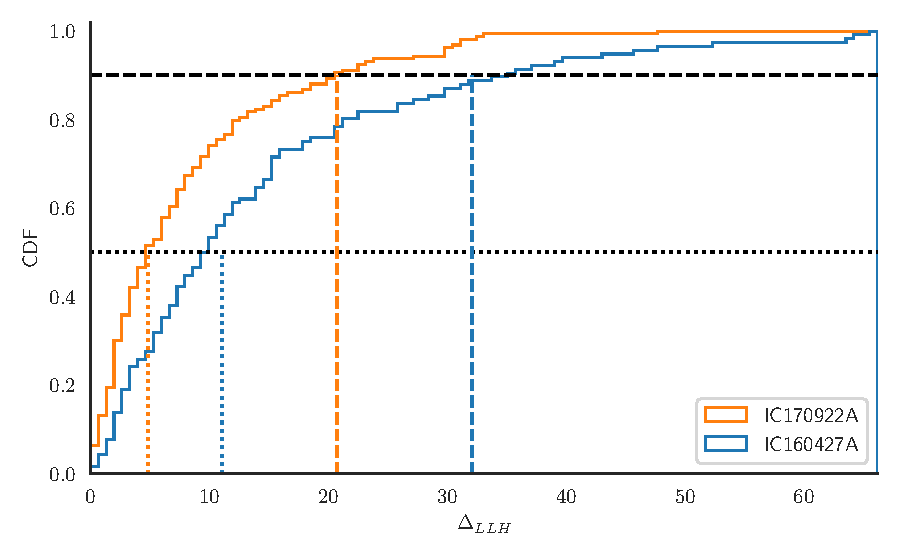
\includegraphics{realtime/resimulations}
	\caption{Cumulative Distribution Functions (CDFs) for the resimulations of \emph{IC160427A} and \emph{IC170922A}.}
	\label{fig:resimulations}
\end{figure}

The outcome of resimulations for two alerts, \emph{IC160427A} and \emph{IC170922A}, can be seen as a Cumulative Distribution Function (CDF) in Figure \ref{fig:resimulations}. 250 resimulated were selected for \emph{IC160427A} \footnote {Of these 250 events, only 117 were available for inclusion in Figure \ref{fig:resimulations}. The remainder have been tragically lost to the sands of time. This explains the offset in critical values from the CDF for this curve.}, while 159 were selected for \emph{IC170922A}. Dotted lines indicate 50\% containment, while dashed lines indicate 90\% containment. For \emph{IC160427A} , 50\% of resimulated events had an LLH offset between best fit and MC truth of 11.1, and 90\% of events within $Delta_{LLH} < 32.1$. By drawing a contour on the likelihood landscape of an alert at $LLH - LLH_{best} = 11.1$ and 32.1, we can say that that the true neutrino arrival direction will lie inside those contours 50\% and 90\% of the time respectively. In comparison, for \emph{IC170922A}, these critical $Delta_{LLH}$ values are somewhat smaller at 4.9 and 20.8 respectively. 

\begin{figure}
	\centering 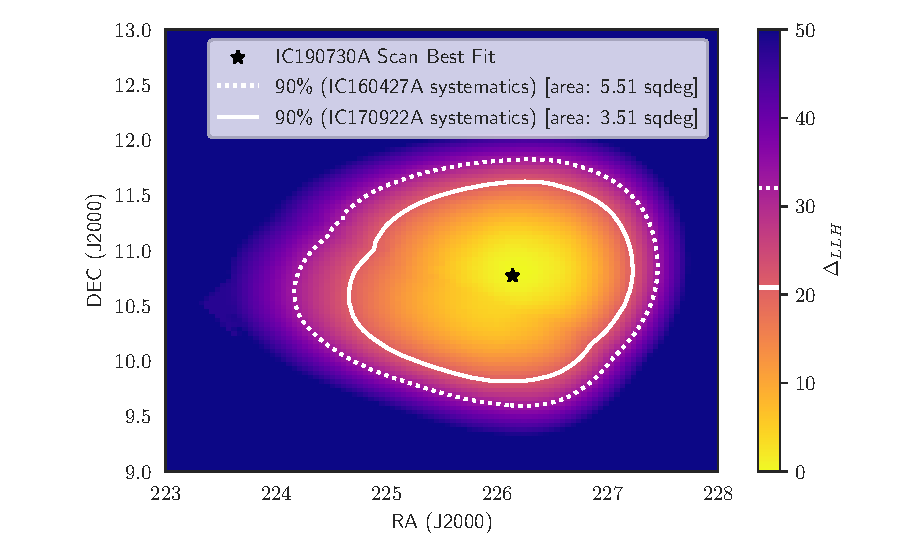
\includegraphics{realtime/contour_IC190730A}
	\caption{An example likelihood contour for \emph{IC190730A}, illustrating both \emph{IC160247A} and \emph{IC170922A} resimulations.}
	\label{fig:ic190730a_contour}
\end{figure}

The resimulation process can take many weeks and thousands of CPU hours, so is generally not performed for each new alert. Instead, the outcome of previous resimulations can be used as a rapid solution. At present, all new alerts are issued using the same resimulations from the first public alert (\emph{IC160427A}, see Section \ref{sec:nu_alerts}). Additional tailored resimulations are employed in a handful of additional cases, though an effort to perform more comprehensive resimulations is planned. A typical contour is shown in Figure \ref{fig:ic190730a_contour}, for \emph{IC190730A}. The contour inferred from the \emph{IC160247A} resimulation is shown in the solid line, while the  \emph{IC170922A} interpretation is dotted. 

\section{Alert Rates}
The alert selections are designed based on Monte Carlo simulations, using the recent IceCube measured astrophysical neutrino flux and spectral index of E$^{-2.19}$ as a signal assumption \sidecite{ic_diffuse_17}. PDFs are then constructed similar to those in Figure \ref{fig:mc_dec_e} of Chapter \ref{ch:llh}, calculating signal/background ratios as a function of energy proxy and reconstructed direction, with thresholds then selected such that the integrated background contamination is <70\% (for bronze) or <50\% (for gold). Each alert is also assigned an individual \emph{signalness} value using the same method, defined as:

\begin{equation}
	signalness(E_{reco}|\theta) = \frac{N_{sig} (E \geq E_{reco}|\theta)}{N_{sig}(E \geq E_{reco}|\theta) + N_{bkg}(E \geq E_{reco}|\theta)}
\end{equation}

The alert rates for each stream can be seen in Table \ref{tab:alert_rates}. Under the V1 alert selection, HESE alerts were issued at a rate of 1.1 signal events per year and 3.7 background alerts per year, while EHE alerts were issued at a rate of 2.48 signal alerts per year and 1.91 background alerts per year \cite{ic_realtime_17}. For V2, Gold alerts were issued at a rate 12.7 per year, while Bronze alerts were issued at a, additional rate of 17.5 per year, yielding a combing rate of one alert per $\sim$2 weeks \cite{ic_realtime_19}. It is clear that the alert rate for V2 is substantially elevated relative to the V1 alert rate.

 \begin{table*}
	\centering
	\begin{tabular}{||c |c |c c| c ||} 
		\hline
		Alert Selection & Stream Name &Signal Rate& Background Rate& Total Rate \\
		& &[yr$^{-1}$]& [yr$^{-1}$]&[yr$^{-1}$]\\
		\hline
		Alerts V1 & HESE & 1.1 & 3.7 & 4.8\\
		& EHE & 2.5 & 1.9 & 4.4\\
		\hline 
		\textbf{Alerts V1}& \textbf{HESE + EHE} & \textbf{3.6} & \textbf{5.6} & \textbf{9.2}\\
		\hline 
		Alerts V2 & Gold & 6.6 & 6.1& 12.7\\
		& Bronze & 2.8 & 14.7& 17.5\\
		\hline 
		\textbf{Alerts V2} & \textbf{Gold + Bronze} & \textbf{9.4} & \textbf{20.8} & \textbf{30.2} \\
		\hline \hline
	\end{tabular}
	\caption{IceCube realtime alert rates.}
	\label{tab:alert_rates}
\end{table*}

\section{Noteworthy IceCube Neutrino Alerts}
\label{sec:nu_alerts}

A summary of all neutrino alerts issued to date is provided in Appendix Table \ref{tab:all_nu_alerts}. Individual neutrino alerts of interest are summarised below. 

\subsection{IC160427A}
\subsubsection*{``The PanSTARRS Supernova Neutrino"}

The first alert issued under this system, HESE alert \emph{IC160427A}  \sidecite{ic160427a}, was found to be in spatial coincidence with an optical transient detected by the Pan-STARRS Observatory while following up the alert \cite{ic_panstarrs_19}. This transient, \emph{PS16cgx} was initially tentatively classified as a Type Ic supernova, for which various models have predicted neutrino emission (see Chapter \ref{ch:sources}).  However, the further spectroscopic and photometric evolution indicated that this was  more likely a Type Ia Supernova, for which no neutrino emission would be expected. 

Given that this was the first HESE alert, and the first high-energy neutrino alert for which a possible counterpart was identified, dedicated resimulations of this event were undertaken following the method in Section \ref{sec:alert_reco}. This was the first characterisation of the impact of systematic uncertainties in modelling the polar glacial ice on directional reconstruction with IceCube for high-energy alerts, and the data from this resimulation continue to be used in all new IceCube alerts. 

\subsection{IC170922A}
\subsubsection*{The ``TXS 0506+056 Neutrino''}
Subsequent neutrino alerts did not yield any probable counterparts, until the detection of EHE alert \emph{IC170922A}\footnote{alternatively named \emph{`The neutrino that launched one thousand telecons'} (Credit: E. Blaufuss)} \sidecite{ic170922a} in spatial coincidence with flaring blazar TXS 0506+056 \sidecite{fermi_txs_atel_17}. After accounting for trial correction from historical neutrino alerts, a chance coincidence was disfavoured at the 3$\sigma$ level \sidecite{ic_txs_mm_18}. The event was also resimulated in the same manner as \emph{IC160427A} . Remarkably, despite its radically-different topology of through-going muon rather than starting track, the results were found to be broadly consistent. More details of TXS 0506+056 are given in Section \ref{subsec:txs}.

\subsection{IC190331A}
\subsubsection*{The``Multi-PeV neutrino''}

A starting track was observed on 2019 March 30th \sidecite{ic190331a}, with a deposited energy of $\sim$5.3 PeV. The initial reconstruction based on \emph{SplineMPE} was inaccurate (for the reasons outlined in Chapter \ref{ch:icecube}., but the update Millipede reconstruction yielded a well-localised position of $\sim$1 sq. deg. on the sky. Given the extraordinarily high deposited energy, and the downgoing starting track topology which disfavours any atmospheric origin (see Chapter \ref{ch:icecube}), IC190331A was one of a handful of track alerts for which an astrophysical origin can be reasonably described as `highly likely'.

\begin{figure}[!ht]
	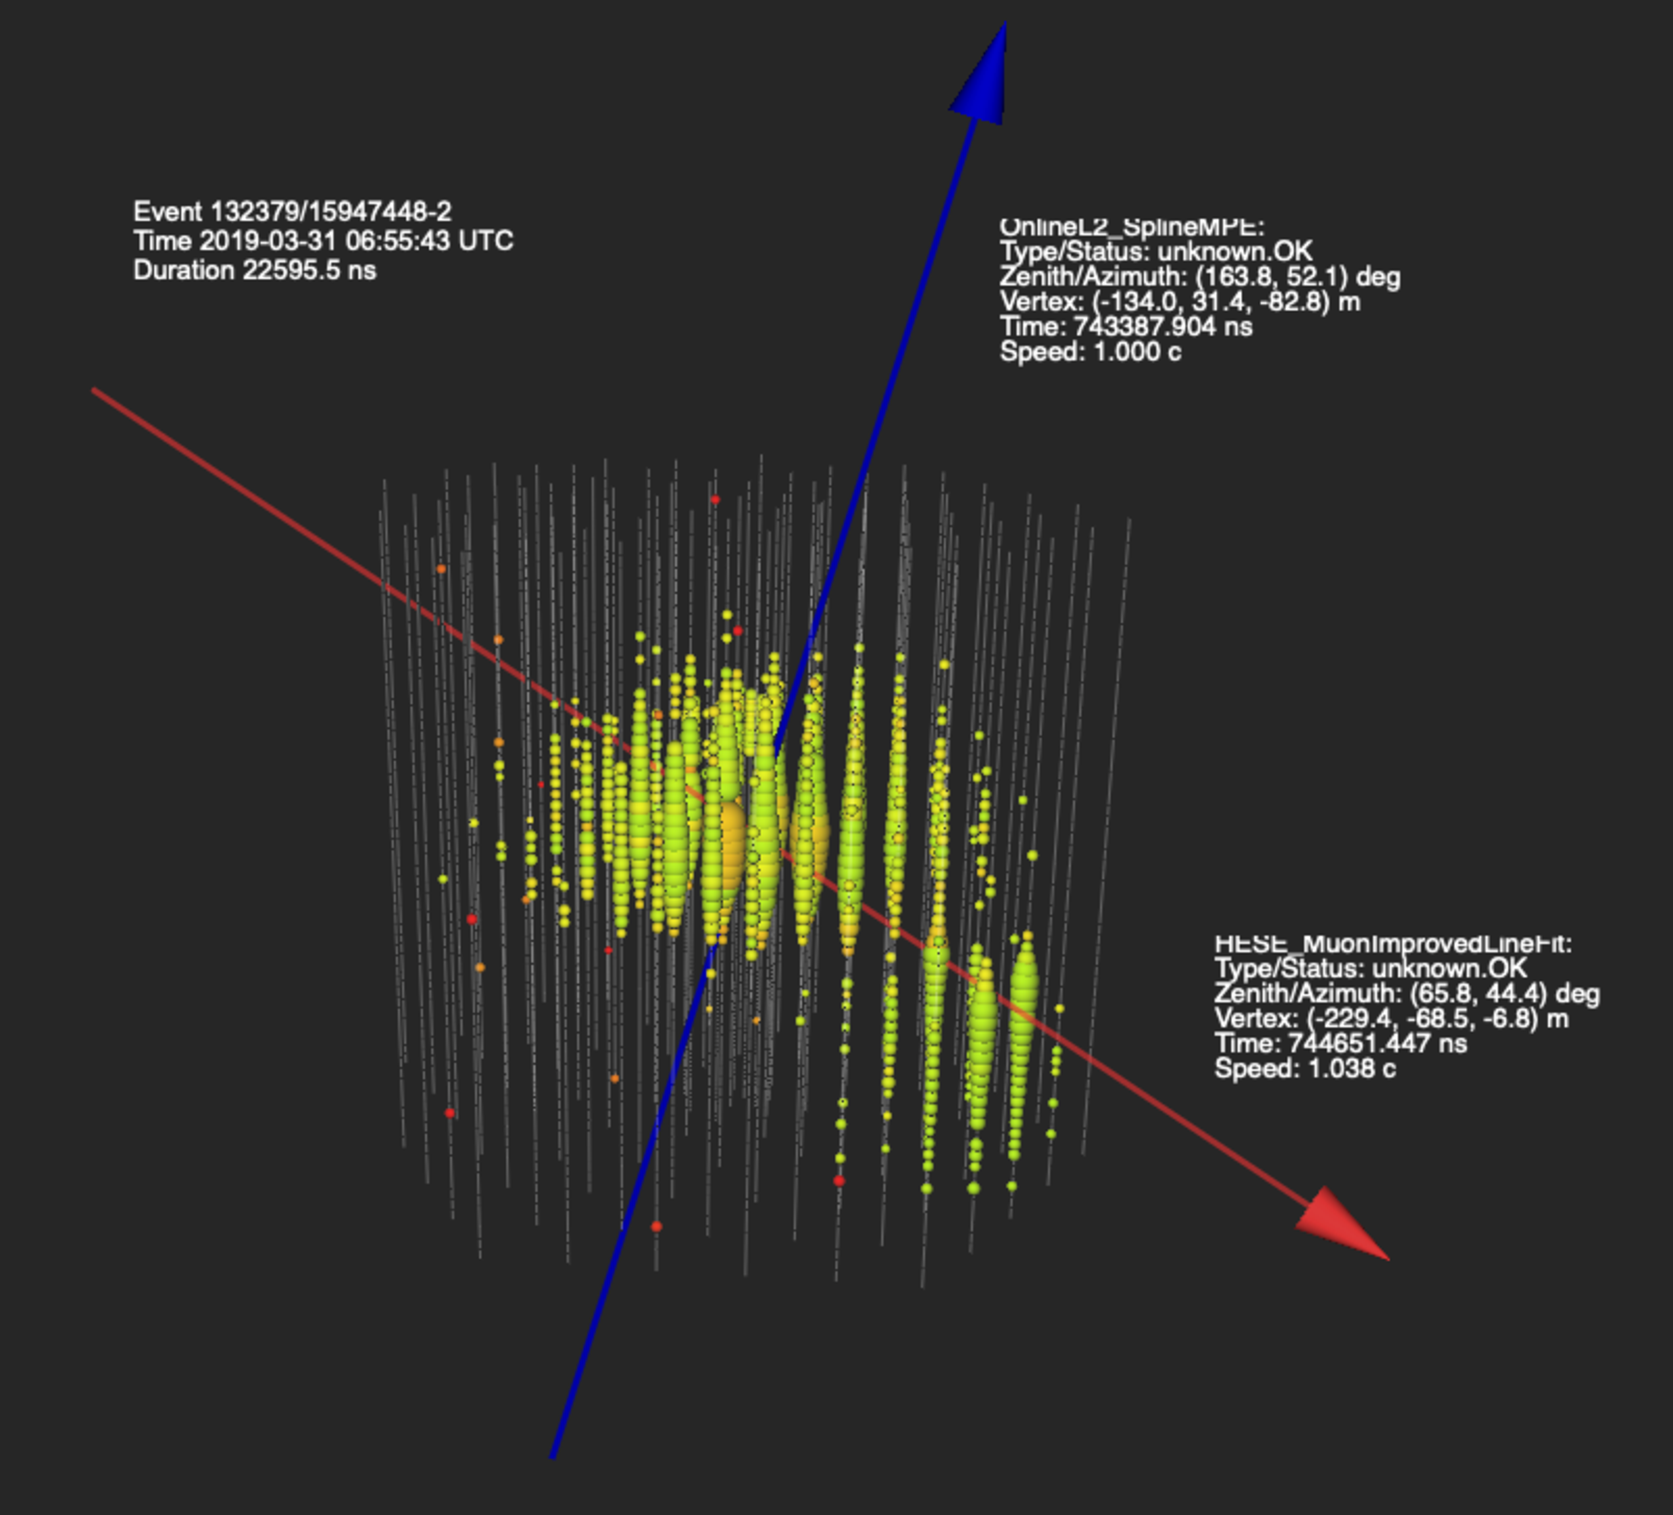
\includegraphics{realtime/ic190331a}
	\caption{Event view of IC190331A. Credit: Cristina Lagunas Gualda}
	\label{fig:ic190331a}
\end{figure}

\subsection{IC190730A}
\subsubsection*{The ``ICRC neutrino''}

\emph{IC190730A} was a golden neutrino alert with a signalness of 67\% \sidecite{ic190730a}, which arrived in the middle of the neutrino astronomy session of the 36th \emph{International Cosmic Ray Conference} (ICRC). Following the automated notice, the full likelihood reconstruction clearly showed it was well-localised, and spatially coincident with FSRQ \emph{PKS 1502+106} (see Chapter \ref{ch:sources}). This particular blazar is extremely bright, being 15th brightest in the sky in terms of integrated gamma-ray energy flux, and owing to its high redshift of z=1.84, is one of the most luminous known blazars \sidecite{franckowiak_20}. This coincidence was reported in the corresponding GCN circular, and triggered a broad multi-wavelength follow-up campaign. 

Though blazar was not found to be flaring in gamma-rays at short timescales \cite{franckowiak_20}, OVRO reported that the radio flux was in recent months elevated relative to the decade long observation baseline \sidecite{ovro_19}. Similar behaviour has been claimed for \emph{TXS 0506+056}, and other neutrino-coincident blazars \cite{ovro_19}. Comprehensive time-dependent modelling has found that the detection of a neutrino alert from \emph{PKS 1502+106} is consistent with the multi-wavelength observations of this object, so a neutrino-blazar association is plausible \sidecite{rodrigues_21}.

%The chance coincidence for at least one neutrino alert to be coincident with any of the  15 brightest blazars was calculated by the author, and found to be disfavoured at the level of 2.n sigma following the procedure in N. 

\subsection{IC190922B }
\subsubsection*{The ``SN2019pqh neutrino''}

On 2019 September 22nd, IceCube for the first time reported multiple high-energy neutrino alerts on a single day. The latter of these was \emph{IC190922B}, a gold alert with a reported signalness of 50.5\% \sidecite{ic190922b}. Follow-up observations of this alert were undertaken by the author with the Zwicky Transient Facility (ZTF), as part of a dedicated neutrino follow-up program introduced in Chapter \ref{ch:ztf_too}. 

One candidate supernova was found, \emph{SN2019pqh}, in spatial and temporal coincidence with the alert \sidecite{ic190922b_atel}. Unlike PS16cgx, this was the first young supernova reported in spatial coincidence with a high-energy neutrino which would be compatible with the CSM-Interaction model introduced in Chapter \ref{ch:sources}. However, as explained in Section \ref{sec:sn2019pqh}, further spectroscopic observations ultimately disfavoured the association. 

\subsection{IC191001A} 
\subsubsection*{The ``Bran Stark neutrino''}

A high-energy gold neutrino event was detected on 2019 October 10, with an estimated signalness of 59\% \sidecite{ic191001a}. A bright Tidal Disruption Event (TDE) \emph{AT2019dsg} was found by the author in spatial coincidence with this alert \sidecite{bran}, as part of follow-up observations using ZTF. This neutrino is explained in much greater detail in Chapter \ref{ch:bran}. As with all ZTF-detected TDEs, AT2019dsg was assigned a nickname inspired by once-popular HBO series \emph{Game of Thrones}, in this case named after character \emph{Bran Stark} \sidecite{van_velzen_20}.

\subsection{IC200107A }
\subsubsection{The``Flaring extreme blazar neutrino''}

\emph{IC200107A} was a high-energy neutrino which passed the initial HESE event selection, but did not qualify as a gold or bronze astrotrack event due to a possible cascade classification \sidecite{ic200107a}. However, visual inspection of the event suggested a starting-track topology, which was confirmed by a dedicated Neutral Network topology classifier \sidecite{ic_dnn_19}. A GCN circular was thus issued to publicise the neutrino arrival direction. However, given the extraordinary nature of the neutrino selection, no signalness estimate was provided.

Two gamma-ray detected blazars were found within the neutrino localisation, \emph{4FGL J0955.1+3551} and \emph{4FGL J0957.8+3423}. The latter of these was not significantly detected at the time of neutrino detection, nor was there any evidence of flaring activity contemporaneous with the neutrino detection. The other blazar \emph{4FGL J0955.1+3551} (also known as \emph{BZB J0955+3551} and \emph{3HSP J095507.9+355101}) belongs to the specific subclass of \emph{extreme blazars}, which are characterised be synchrotron peaks at very high-frequencies, which had been proposed as especially promising candidates of high-energy neutrinos \sidecite{padovani_16}. Follow-up observations by \emph{Swift}-XRT of the source revealed a dramatic simultaneous X-ray flare \sidecite{krauss_ic200107a, giommi_ic200107a}, of particular interest because of the importance of X-ray photons in the p$\gamma$ neutrino production models introduced in Chapter \ref{ch:theory}.

More comprehensive multi-frequency modelling has confirmed that the detection of a neutrino alert from an extreme blazar is realistic, though the simultaneous X-ray flare may not be directly related to neutrino production \sidecite{paliya_20, giommi_20, petropoulou_20}. The probability for chance coincidence of the neutrino alert with an extreme blazar flaring in X-rays was calculated by the author of this thesis to be 3.7 $\times 10^{-3}$, but in the absence of any systematic X-ray blazar follow-up program it is unclear how this number could be trial corrected (see Chapter \ref{ch:llh}) \cite{paliya_20}. The statistical evidence for this association is thus insufficient to draw any definitive conclusions about the neutrino origin.

\subsection{IC200530A}
\subsubsection{The "Tywin Lannister neutrino"}

\emph{IC200530A} was a high-energy gold alert detected on 2020 May 30th, with a signalness estimate of 59\% \sidecite{ic200530a}. The neutrino was also observed as part of the ZTF neutrino follow-up program, and the bright nuclear flare \emph{AT2019fdr} was identified by the author as a probable optical counterpart \sidecite{ic200530a_ztf}. The object was later classified as a likely TDE \sidecite{frederick_20}, the second found in spatial and temporal coincidence with a high-energy neutrino. More details on this object are given in Section \ref{sec:at2019fdr}. The ZTF-assigned Game of Thrones name was \emph{Tywin Lannister}.